\documentclass{beamer}
\usepackage{graphicx}
\usepackage{hyperref}

\title{Introduction to Multi-Agent Reinforcement Learning}
\author{Julien Soulé}
\institute{$CO^{4}SYS$ Team, LCIS Lab}
\date{\today}

\begin{document}

% Title Slide
\begin{frame}
  \titlepage
\end{frame}

% Foreword
\section*{Foreword}
\begin{frame}{Foreword}
  \begin{figure}
    \centering
    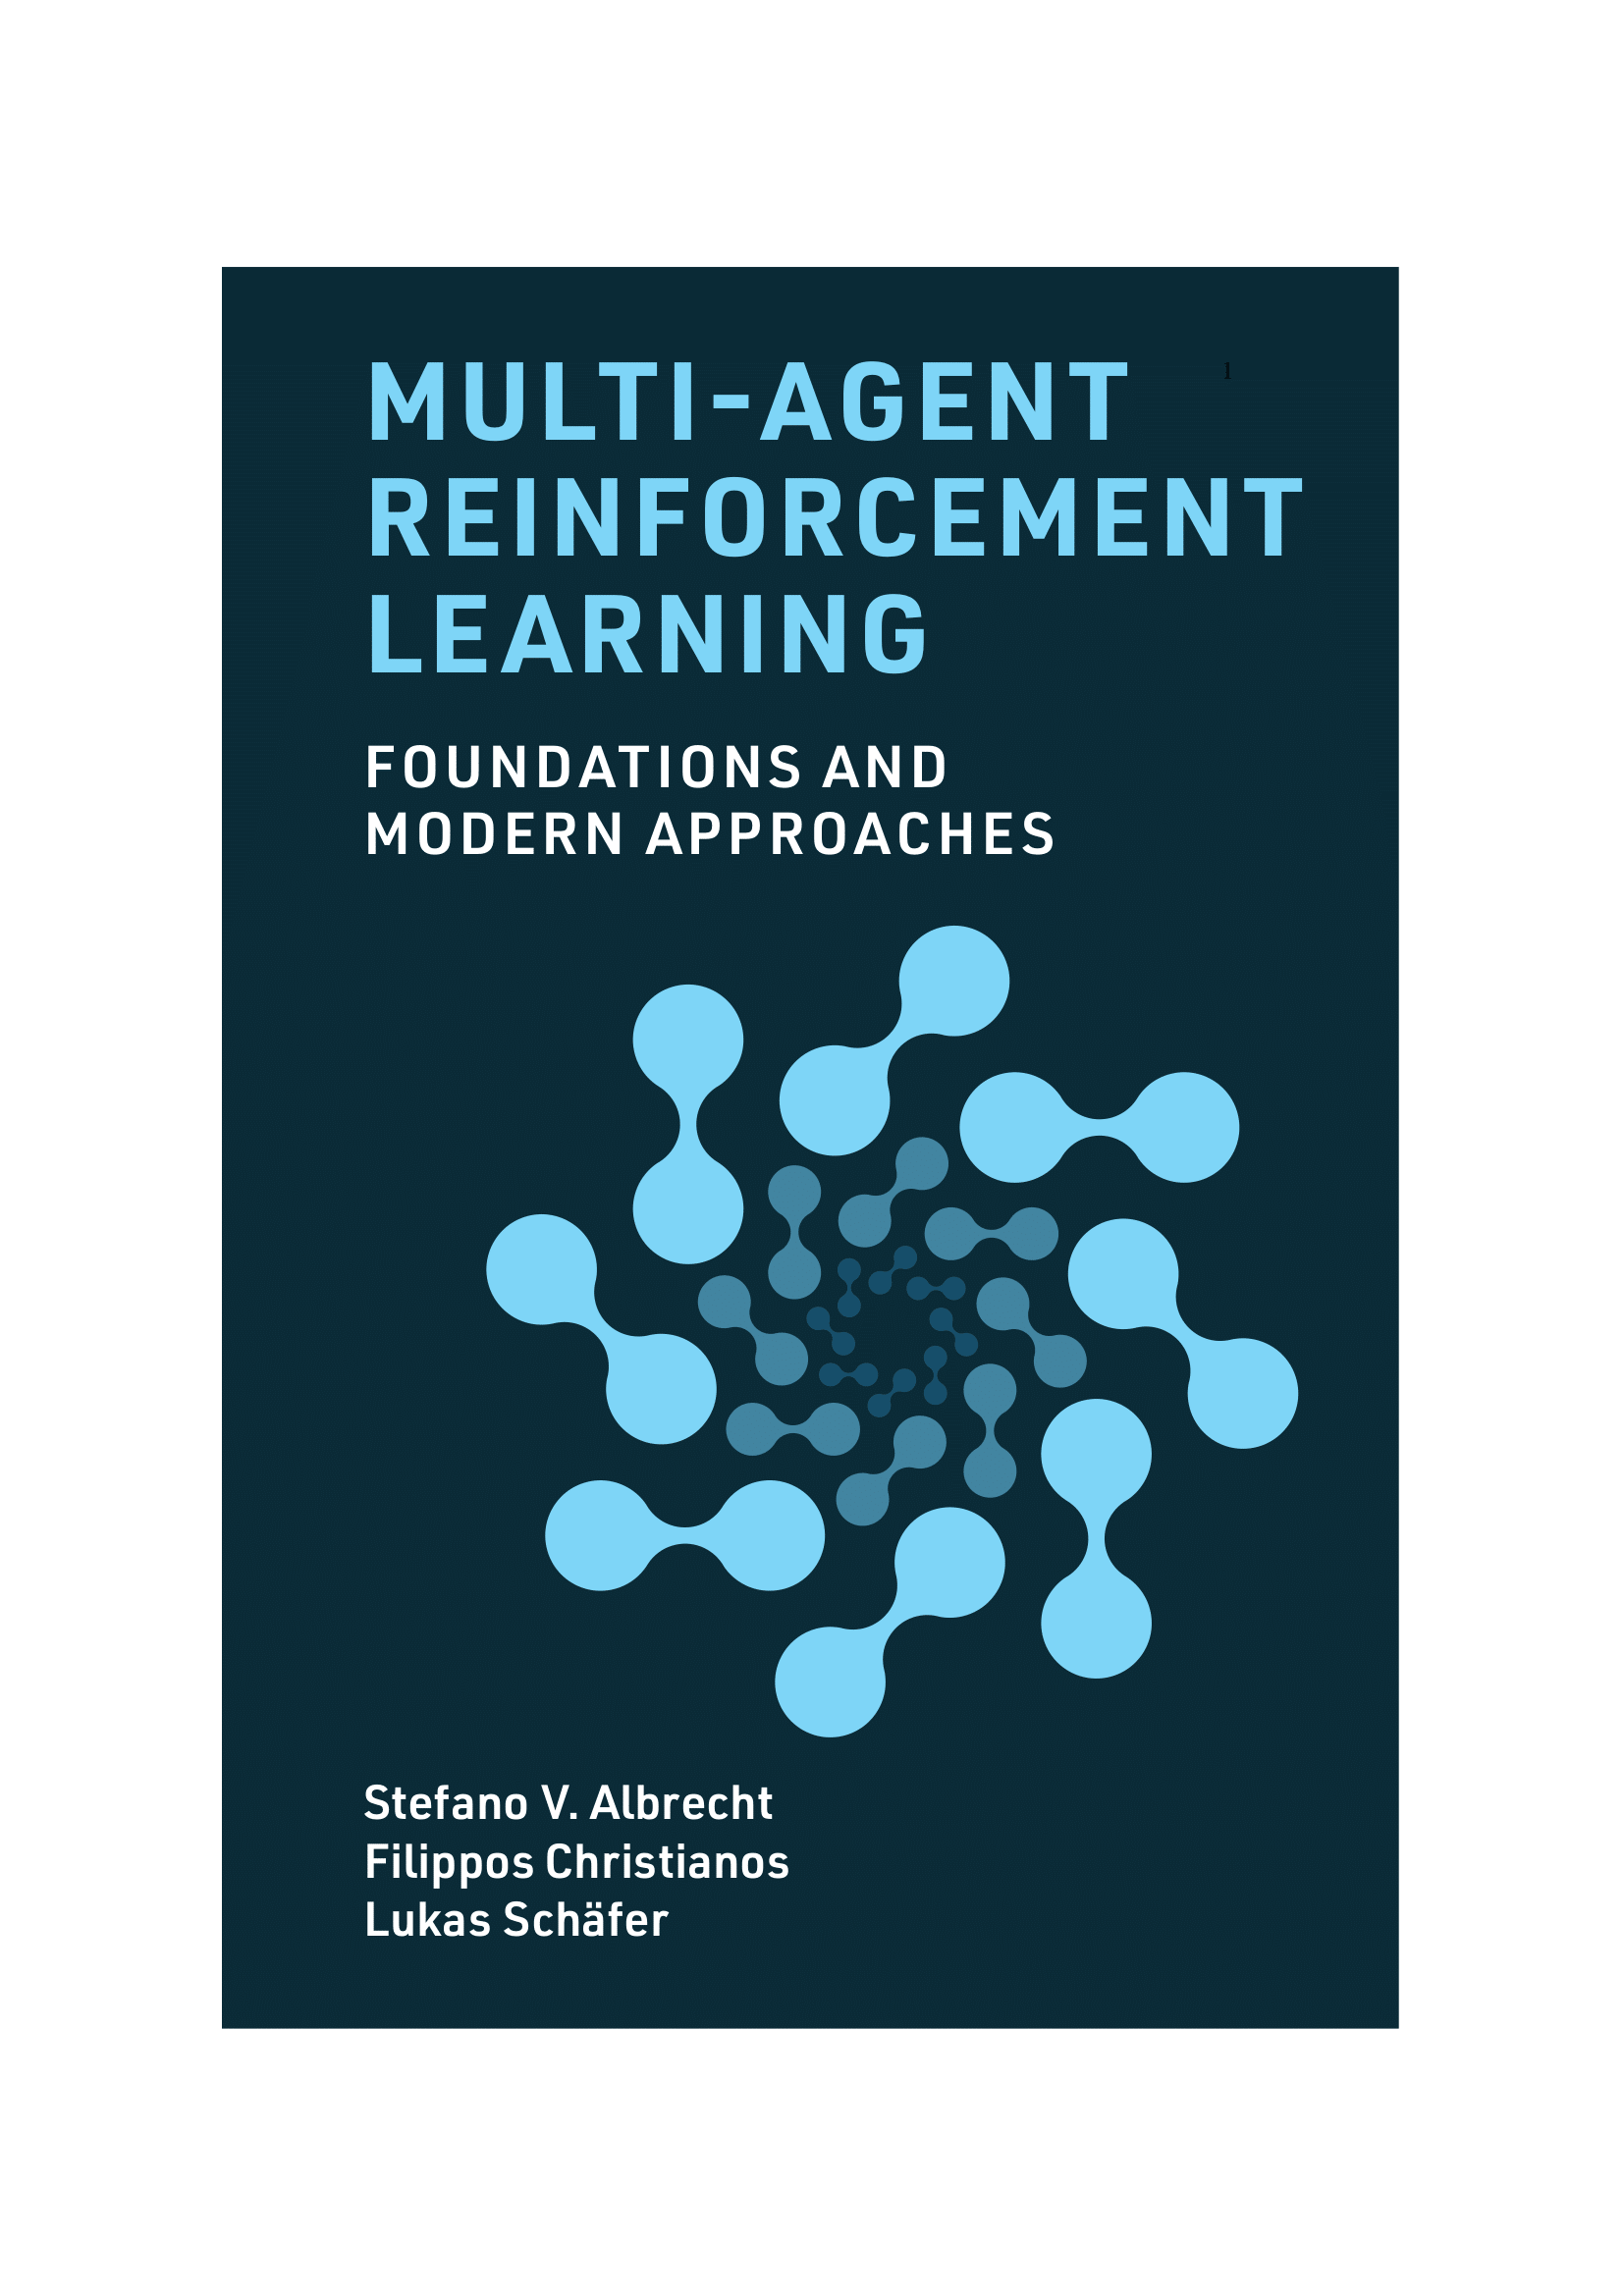
\includegraphics[width=0.45\textwidth]{figures/marl-book-cover.png}
    \caption{Stefano V. Albrecht, Filippos Christianos, and Lukas Schäfer. Multi-Agent Reinforcement Learning: Foundations and Modern Approaches. MIT Press, 2024.}
  \end{figure}
\end{frame}

% Table of Contents
\begin{frame}{Table of Contents}
  \tableofcontents
\end{frame}

% Chapter 1: Introduction
\section{Introduction}

\begin{frame}{Multi-Agent Reinforcement Learning (MARL)}
  \begin{itemize}
    \item Overview of MARL
    \item Agents interacting in a shared environment
    \item Focus on learning optimal policies
  \end{itemize}
\end{frame}

\begin{frame}{Applications of MARL}
  \begin{itemize}
    \item Multi-Robot Warehouse Management
    \item Competitive Play in Board Games and Video Games
    \item Autonomous Driving
    \item Automated Trading in Electronic Markets
  \end{itemize}
\end{frame}

\section{Foundations of MARL}

% Chapter 2: Reinforcement Learning
\subsection{Reinforcement Learning}
\begin{frame}{Reinforcement Learning}
  \begin{itemize}
    \item Definition and key concepts
    \item Markov Decision Processes (MDPs)
    \item Optimal policies and value functions
  \end{itemize}
\end{frame}

% Chapter 3: Games - Models of Multi-Agent Interaction
\subsection{Games: Models of Multi-Agent Interaction}
\begin{frame}{Game Models}
  \begin{itemize}
    \item Normal-Form Games
    \item Stochastic Games
    \item Partially Observable Stochastic Games
  \end{itemize}
\end{frame}

% Chapter 4: Solution Concepts for Games
\subsection{Solution Concepts for Games}
\begin{frame}{Solution Concepts for Games}
  \begin{itemize}
    \item Nash Equilibrium and $\epsilon$-Nash Equilibrium
    \item Pareto Optimality
    \item Social Welfare and Fairness
  \end{itemize}
\end{frame}

% Chapter 5: First Steps and Challenges in MARL
\subsection{First Steps and Challenges in MARL}
\begin{frame}{Challenges in MARL}
  \begin{itemize}
    \item Non-stationarity
    \item Equilibrium Selection
    \item Multi-Agent Credit Assignment
  \end{itemize}
\end{frame}

% Part II: Multi-Agent Deep Reinforcement Learning
\section{Multi-Agent Deep Reinforcement Learning}

% Chapter 7: Deep Learning
\subsection{Deep Learning}
\begin{frame}{Deep Learning}
  \begin{itemize}
    \item Neural Networks
    \item Convolutional and Recurrent Networks
    \item Backpropagation and Optimization
  \end{itemize}
\end{frame}

% Chapter 8: Deep Reinforcement Learning
\subsection{Deep Reinforcement Learning}
\begin{frame}{Deep Reinforcement Learning}
  \begin{itemize}
    \item Deep Q-Networks (DQN)
    \item Policy Gradient Algorithms
    \item Actor-Critic Methods
  \end{itemize}
\end{frame}

% Chapter 9: Multi-Agent Deep Reinforcement Learning
\subsection{Multi-Agent Deep Reinforcement Learning}
\begin{frame}{Multi-Agent Deep Reinforcement Learning}
  \begin{itemize}
    \item Centralized vs. Decentralized Training
    \item Multi-Agent Policy Gradient Theorem
    \item Value Decomposition Methods
  \end{itemize}
\end{frame}

% Chapter 10: MARL in Practice
\subsection{MARL in Practice}
\begin{frame}{MARL in Practice}
  \begin{itemize}
    \item MARL Neural Networks in PyTorch
    \item Practical Tips for MARL Algorithms
    \item Presentation of Experimental Results
  \end{itemize}
\end{frame}

% Conclusion
\section{Conclusion}
\begin{frame}{Conclusion}
  \begin{itemize}
    \item Summary of Key Concepts
    \item Open Challenges in MARL
    \item Future Directions in Research
  \end{itemize}
\end{frame}

\end{document}
